%%
%% Kapitel
%%
\chapter{Sprachmodelle}
Bis zur Einf\"uhrung von Sprachmodellen gab es f\"ur NLP in Machine Learning ein gro{\ss}es Problem: Textdaten, wie auch Sprache, sind inherent sequentiell. Im Gegensatz zu Bildern, bei denen alle Daten auf einmal verarbeitet werden k\"onnen, konnte die Textverarbeitung die Beschleunigung durch den Einsatz von GPUs nicht nutzen, da viele Aufgaben nicht parallelisiert werden konnten \cite{attention}.\\ Weiterhin gab es keine M\"oglichkeit, ein schon vortrainiertes Modell f\"ur andere Aufgaben weiter zu verwenden, da das Training f\"ur die verschiedenen Aufgaben und auch Dom\"anen sehr spezifisch angegangen werden muss. Diese Faktoren f\"uhrten zu einem deutlichen Mehraufwand von NLP z.B. gegen\"uber Bildverarbeitung.\\
Das Ziel von Sprachmodellen ist es, parallele Verarbeitung der Daten m\"oglich zu machen sowie, im Gegensatz zu vortrainierten \textbf{Wortvektor Embeddings} wie \textbf{GLoVe} den Kontext der einzelnen W\"orter im Satz zu wahren. In den Embeddings wird jedem Wort ein Vektor zugewiesen, sodass \"ahnliche W\"orter nah beieinander liegen und die Beziehung zwischen W\"ortern erhalten bleibt. Dadurch k\"onnen interessante Rechnungen aufgestellt werden:
\begin{verbatim} 
London - England + Spanien = Madrid
\end{verbatim} 
Mit ganzen Textsequenzen k\"onnen aber auch diese Vektor Embeddings aufgrund der fehlenden Kontextinformationen nur bedingt gut umgehen.


\section{Vergleich zu anderen Ans\"atzen}
Wie schon erw\"ahnt muss Sprache sequentiell versarbeitet werden. Dazu werden meist \textbf{Gated RNNs} und \textbf{Long Short Term Memory (LSTM)} - Netzwerke verwendet \cite{attention}. Durch einige Techniken kann man mit diesen Netzen auch gute Laufzeiten erreichen, aber es besteht ein weiteres Problem: Der Kontext der W\"orter geht verloren. Zwar k\"onnen \textbf{LSTMs} gut mit kurzen S\"atzen umgehen, aber je l\"anger die Wortsequenz, desto schlechter kann sie verarbeitet werden: Es gibt dabei Probleme mit \textbf{vanishing} oder \textbf{exploding gradients}, je nach Einstellung der Parameter.\\
Durch die sequentiellen Verarbeitung steigt auch die Verarbeitungszeit mit der Textl\"ange an, wobei \textbf{LSTMs} generell langsamer sind als \textbf{RNNs}, da die Neuronen komplexer sind.\\
Der Umstand, dass diese Netze f\"ur jede Anwendung spezifisch trainiert werden m\"ussen, macht ihren Einsatz sehr umst\"andlich. Sprachmodelle hingegen sind vortrainiert, sie brauchen nur eine geringe Anzahl Daten und damit auch wenig Zeit, um f\"ur verschiedene Anwendungen einsatzbereit zu sein.


\section{Transformer}
\textbf{Transformer} sind die Basis vieler der heutigen Sprachmodelle \cite{bert}\cite{gpt}. Sie wurden 2017 entwickelt, um das Problem der sequentiellen Verarbeitung zu l\"osen: Als Eingabe kann ein \textbf{Transformer} eine ganze Textsequenz verarbeiten.\\
\begin{figure}
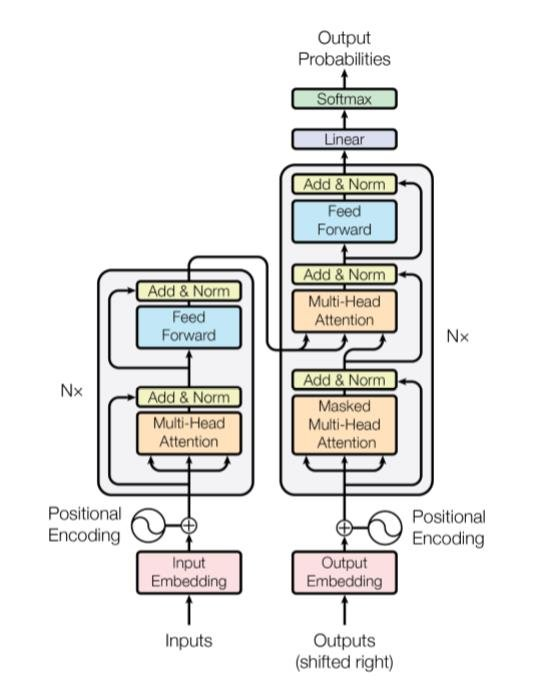
\includegraphics[width=\linewidth]{pics/attention.jpg}
\caption{Abb. 1: Aufbau eines Transformers \cite{attention}}
\label{fig:attention}
\end{figure}
%Encoder
Wie in \ref{fig:attention} zu sehen, wird die Eingabe zun\"achst in Wortvektoren f\"ur jedes Eingabewort umgewandelt, die sich aus der Addition des Vektors im \textbf{Embedding Space} mit einem \textbf{Positionsvektor (Positional Encoding)}, der die Position des Wortes im Satz enth\"alt, ergibt. Der Positionsvektor wird durch Sinus- und Kosinusfunktionen bestimmt. Dieser Eingabevektor wird an einen \textbf{Encoder} weitergegeben, der eine \textbf{Attention-Matrix} f\"ur die Eingabesequenz erstellt. Sie besteht aus einem Vektor der L\"anger der Textsequenz f\"ur jedes Wort. Diese Matrix enth\"alt Informationen dar\"uber, wie relevant die einzelnen W\"orter der Sequenz f\"ureinander sind: In dem Satz
\begin{verbatim} 
Der braune Hund
\end{verbatim} 
bezieht sich z.B. das Wort "`Der"' sowie das Adjektiv "`braune"' auf das Wort "`Hund"'. In dem Attention-Vektor w\"aren entsprechend die Werte f\"ur "`Hund"' in den Vektoren der beiden anderen W\"orter h\"oher. \textbf{Attention} ist der Schl\"usselpunkt f\"ur die Funktion der Transformer: Dadurch erhalten die Wortvektoren ihre eigentliche Kontextinformation.\\
Alle bisher errechneten Vektoren werden danach aufaddiert, normalisiert und jeder Vektor wird in ein Feed-Forward-Netz gegeben. Hierbei kann parallelisiert werden, da die einzelnen Vektoren voneinander unabh\"angig sind. Die Ausgabe des \textbf{Encoders} sind die mit Kontext und Attention encodierten Wortvektoren.\\
%Decoder 

\section{GPT}


\section{ELMo}

\section{BERT}
%Unterschied zu anderen Modellen
%verschiedene Trainingsmethoden


\section{ULMFit}
%Unterschied zu anderen Modellen